\documentclass[11pt,a4paper]{article}

% ---------------------------------------------------------------
% Packages
% ---------------------------------------------------------------
\usepackage[T1]{fontenc}
\usepackage[utf8]{inputenc}
\usepackage{lmodern}
\usepackage[a4paper,margin=2.5cm]{geometry}
\usepackage{amsmath,amssymb,bm}
\usepackage{booktabs,tabularx,array}
\usepackage{siunitx}
\usepackage{enumitem}
\usepackage{xcolor}
\usepackage{graphicx}
\usepackage[numbers,sort&compress]{natbib}
\usepackage[colorlinks=true,linkcolor=blue!50!black,citecolor=blue!50!black,urlcolor=blue!50!black]{hyperref}

\sisetup{range-phrase=--, range-units=single}
\newcolumntype{L}{>{\raggedright\arraybackslash}X}
\renewcommand{\arraystretch}{1.2}
\newcommand{\todo}[1]{\textcolor{red!70!black}{\textbf{Open:} #1}}

% ---------------------------------------------------------------
% Title
% ---------------------------------------------------------------
\title{GREAT Cell -- THM Model Description}
\author{Olaf Kolditz\\Helmholtz Centre for Environmental Research -- UFZ}
\date{7 November 2026}

\begin{document}
\maketitle

\begin{abstract}
This report describes the coupled thermo-hydro-mechanical (THM) model used to
simulate the GREAT cell experiments in OpenGeoSys. It covers the experimental
apparatus, governing equations, constitutive models, geometry and boundary
conditions, numerical implementation, benchmark stages, and the main
assumptions and open points.
\end{abstract}

\tableofcontents

% ---------------------------------------------------------------
\section{Purpose and scope}
% ---------------------------------------------------------------
The THM model reproduces the coupled thermal, hydraulic and mechanical response
of rock samples tested in the GREAT cell, so that simulated stresses, strains,
pore pressures and temperatures can be compared directly with the cell's sensor
data. It serves three goals:
\begin{itemize}
  \item \textbf{Verification and validation} of coupled THM codes (primarily
        OpenGeoSys) against a well-controlled, true-triaxial laboratory experiment.
  \item \textbf{Interpretation} of the measured strain field and injection
        pressures, including the stress redistribution around a central borehole
        and a fracture.
  \item \textbf{Benchmarking} within the international DECOVALEX framework,
        where several teams model the same experimental stages~\cite{UFZDecovalex2023}.
\end{itemize}
The model covers the intact sample (poroelastic, thermo-poroelastic) and the
fractured sample (fluid flow in a single fracture under polyaxial stress).

% ---------------------------------------------------------------
\section{Background and literature}
% ---------------------------------------------------------------
The GREAT cell was introduced by McDermott et al.~\cite{McDermott2018} as a
true-triaxial cell for \SI{200}{mm} samples that rotates the stress field
without moving the sample and records surface strain with distributed fibre
optics. First hydro-mechanical tests on resin analogues showed that fracture
permeability follows the normal stress on the fracture as the load rotates.

Within DECOVALEX, the GREAT cell is one of the reference experiments of the
SAFENET task, which brought fracture mechanics into DECOVALEX for the first
time~\cite{UFZDecovalex2023}. Kolditz et al.~\cite{Kolditz2025} describe the
follow-up task SAFENET-2 (DECOVALEX~2027), which extends and validates the
models from the laboratory to the field scale. It combines a hydro-mechanical
route based on GREAT cell tests on Greywacke and Gneiss with a
thermo-mechanical route (thermally induced slip and permeability change in
fractured granite), and links both to the STIMTEC in-situ experiment at the
Reiche Zeche mine in Freiberg. The GREAT cell has since been fitted with a
heater, which makes thermal stages such as those modelled here possible.

Mollaali et al.~\cite{Mollaali2026} define the numerical benchmarks for the
GREAT cell: a 2D plane-strain section with rubber sheath, PEE and DSS loads
(load cases A, B, C, E and F), and stages from intact mechanical loading to injection and
fracture propagation. They compare a discrete approach with lower-dimensional
interface elements and a smeared phase-field approach in OpenGeoSys. The
present THM model uses their geometry, Load~A and rock parameters, and adds
the heating and injection phases of the T and TH models.

% ---------------------------------------------------------------
\section{The GREAT cell experiment}
% ---------------------------------------------------------------
The GREAT cell (Geo-Reservoir Experimental Analogue Technology) loads a
\SI{200}{mm} $\times$ \SI{200}{mm} cylindrical sample with a true-triaxial,
rotatable stress field while fluid flows through it and fibre optics record
surface strain~\cite{McDermott2018,EdinburghGREAT}. Table~\ref{tab:apparatus}
summarises the apparatus.

\begin{table}[htbp]
\centering
\caption{GREAT cell specification~\cite{McDermott2018}.}
\label{tab:apparatus}
\begin{tabularx}{\textwidth}{@{}lL@{}}
\toprule
Feature & Specification \\
\midrule
Sample           & Cylinder, $\sim$\SI{200}{mm} diameter $\times$ \SI{200}{mm} length \\
Radial loading   & 8 opposing pairs of fluid-filled pressure-exerting elements (PEEs); each pair shares one pump \\
Seals between PEEs & Dynamic sealing strips (DSS) \\
Sleeve           & \SI{2}{mm} Viton (fluoroelastomer) sheath between sample and PEEs/DSS \\
Design limits    & \SI{100}{MPa} radial and axial stress, \SI{40}{MPa} pore pressure, \SI{100}{\celsius} \\
Stress rotation  & Changing PEE pressures rotates the field without moving the sample \\
Heating          & Electro-resistance bands around the cell body in an insulating jacket; thermocouples on inlet and outlet lines \\
Strain sensing   & Distributed fibre optics (LUNA ODiSI-B) in a $<$\SI{1}{mm} groove; a value every \SI{2.5}{mm}, \SI{25}{Hz} \\
Fluid access     & Ports in the top platen (centre and \SI{50}{mm} radius); central borehole for injection \\
\bottomrule
\end{tabularx}
\end{table}

The first tests used polymer and resin analogues (stiffness $\sim$\SI{3.85}{GPa}
and $\sim$\SI{4.3}{GPa}) at \SIrange{2}{10}{MPa} rotating loads and fracture
fluid pressures up to $\sim$\SI{4}{MPa}. Later campaigns and the benchmarks use
Greywacke and Gneiss~\cite{Mollaali2026}.

% ---------------------------------------------------------------
\section{Governing equations}
% ---------------------------------------------------------------
The model is quasi-static, fully saturated, single-phase Biot poro-elasticity
extended by heat transport. Primary variables are displacement $\mathbf{u}$,
pore pressure $p$ and temperature $T$.

\paragraph{Momentum balance} with Biot effective stress and thermal strain:
\begin{equation}
  \nabla \cdot \left( \bm{\sigma}' - \alpha_B \, p \, \mathbf{I} \right) + \rho \mathbf{g} = \mathbf{0},
  \qquad
  \bm{\sigma}' = \mathbb{C} : \left( \bm{\varepsilon} - \alpha_T (T - T_0)\, \mathbf{I} \right)
\end{equation}

\paragraph{Fluid mass balance} in the rock matrix (Darcy flow):
\begin{equation}
  S \, \frac{\partial p}{\partial t}
  + \alpha_B \, \frac{\partial (\nabla\cdot\mathbf{u})}{\partial t}
  - \beta_{\mathrm{eff}} \frac{\partial T}{\partial t}
  - \nabla \cdot \left( \frac{\mathbf{k}}{\mu} \left( \nabla p - \rho_f \mathbf{g} \right) \right) = Q_f
\end{equation}

\paragraph{Fluid flow in a fracture} (lubrication approximation, cubic law with
hydraulic aperture $w$):
\begin{equation}
  \frac{\partial w}{\partial t} + w\, S_f \frac{\partial p}{\partial t}
  - \nabla_{\Gamma} \cdot \left( \frac{w^3}{12\,\mu} \nabla_{\Gamma} p \right) = q_{\mathrm{leak}}
\end{equation}

\paragraph{Energy balance} (conduction and advection, local thermal equilibrium):
\begin{equation}
  (\rho c_p)_{\mathrm{eff}} \frac{\partial T}{\partial t}
  + \rho_f c_{p,f} \, \mathbf{q} \cdot \nabla T
  - \nabla \cdot \left( \lambda_{\mathrm{eff}} \nabla T \right) = Q_T
\end{equation}

Here $S$ is the storage coefficient, $\alpha_B$ the Biot coefficient, $\alpha_T$
the linear thermal expansion coefficient, $\beta_{\mathrm{eff}}$ the effective
thermal expansion of the pore space, $\mathbf{k}$ the permeability tensor, $\mu$
the viscosity, $\mathbf{q}$ the Darcy flux and $\lambda_{\mathrm{eff}}$ the
effective thermal conductivity. Purely mechanical and hydro-mechanical stages
are special cases with $T$ held constant.

% ---------------------------------------------------------------
\section{Constitutive models and material parameters}
% ---------------------------------------------------------------
Rock and sheath are linear-elastic and isotropic; fractures are represented
either discretely or smeared~\cite{Mollaali2026} (Table~\ref{tab:constitutive}).

\begin{table}[htbp]
\centering
\caption{Constitutive models.}
\label{tab:constitutive}
\begin{tabularx}{\textwidth}{@{}lLL@{}}
\toprule
Component & Constitutive model & Key parameters \\
\midrule
Rock matrix (Greywacke, Gneiss) & Linear isotropic (thermo-)poro-elasticity
  & $E$, $\nu$, $\rho$, $\phi$, $k$, $\alpha_B$, $\alpha_T$, $\lambda$, $c_p$ \\
Viton sheath & Linear elastic, impermeable & $E$, $\nu$ (much softer than the rock) \\
Fracture, discrete (LIE) & Joint law $\mathrm{d}\bm{\sigma}_f = \mathbf{K}\,\mathrm{d}\mathbf{w}$ with normal, shear and coupling stiffness $k_{nn}$, $k_{tt}$, $k_{nt}$
  & Initial aperture $w_0$, $k_{nn}$, $k_{tt}$ \\
Fracture, smeared (VPF) & Phase-field damage (AT1/AT2), $\mathbf{K}_v = K_m\mathbf{I} + (1-v)\,\xi\,\frac{w^3}{12}(\mathbf{I}-\mathbf{n}\otimes\mathbf{n})$
  & Length scale $\ell$, toughness $G_c$, aperture $w \approx h_e \varepsilon_1$ \\
Fluid (water) & Constant or $T$-dependent $\rho_f$, $\mu$ & $\rho_f$, $\mu$, compressibility, $c_{p,f}$, $\lambda_f$ \\
\bottomrule
\end{tabularx}
\end{table}

Greywacke is the softer and more compressible rock; Gneiss is stiffer and
tighter. Table~\ref{tab:params} lists the values used in the THM model for
Load~A (\texttt{THM\_model/make\_THM\_prj.py}); elasticity, Biot coefficient,
porosity and solid density follow Table~1 of~\cite{Mollaali2026}.

\begin{table}[htbp]
\centering
\caption{Material parameters of the THM model.}
\label{tab:params}
\small
\begin{tabular}{@{}lccc@{}}
\toprule
Parameter & Greywacke & Gneiss & Sheath \\
\midrule
Young's modulus $E$ (GPa)            & 26.85 & 83.9 & 0.1 \\
Poisson's ratio $\nu$ (--)           & 0.27  & 0.21 & 0.4 \\
Solid density $\rho_s$ (kg\,m$^{-3}$) & 2650  & 2750 & 1200 \\
Porosity $\phi$ (--)                 & 0.005 & 0.001 & as rock \\
Biot coefficient $\alpha_B$ (--)     & 0.8   & 0.6  & 0 \\
Permeability $k$ (m$^2$)             & \multicolumn{3}{c}{$1.409\times10^{-14}$ (rock and sheath)} \\
Bulk thermal conductivity $\lambda$ (W\,m$^{-1}$\,K$^{-1}$) & \multicolumn{3}{c}{2.8} \\
Bulk heat capacity $\rho c$ (J\,m$^{-3}$\,K$^{-1}$) & \multicolumn{3}{c}{$2700 \times 790$} \\
Linear thermal expansion $\alpha_T$ (K$^{-1}$) & \multicolumn{3}{c}{$8\times10^{-6}$ (solid)} \\
\midrule
\multicolumn{4}{@{}l}{Water: $\rho_f = 1000$ kg\,m$^{-3}$, $\beta_f = 4.4\times10^{-10}$ Pa$^{-1}$, $\mu = 10^{-3}$ Pa\,s,} \\
\multicolumn{4}{@{}l}{\phantom{Water: }$c_f = 4180$ J\,kg$^{-1}$\,K$^{-1}$, $\lambda_f = 0.6$ W\,m$^{-1}$\,K$^{-1}$, no thermal expansion} \\
\bottomrule
\end{tabular}
\end{table}

The solid conductivity and heat capacity are back-calculated from the bulk
values for each porosity. Storage is not set directly; it follows from $\phi$,
$\alpha_B$, $\beta_f$ and the elasticity.

% ---------------------------------------------------------------
\section{Geometry, mesh and boundary conditions}
% ---------------------------------------------------------------
\subsection{Geometry}
The model is a 2D plane-strain horizontal mid-section of the sample
(Fig.~\ref{fig:geometry}): a rock disc of radius \SI{0.097}{m} (MaterialID~0)
inside a \SI{3}{mm} rubber sheath up to $r=\SI{0.100}{m}$ (MaterialID~1). The
outer boundary is split into 16 PEE arcs and 16 DSS arcs. PEE~1 is centred at
\ang{0}, PEE~$i$ at $-(i-1)\times\ang{22.5}$ (clockwise), and PEE~$i$a lies
opposite at $+\ang{180}$. Each PEE arc spans \ang{18} and each DSS arc
\ang{4.5}; these widths are estimated from Fig.~4b of~\cite{Mollaali2026}.
A probe circle at $r=\SI{0.065}{m}$ records volumetric strain, and the centre
node carries the injection.

\begin{figure}[htbp]
\centering
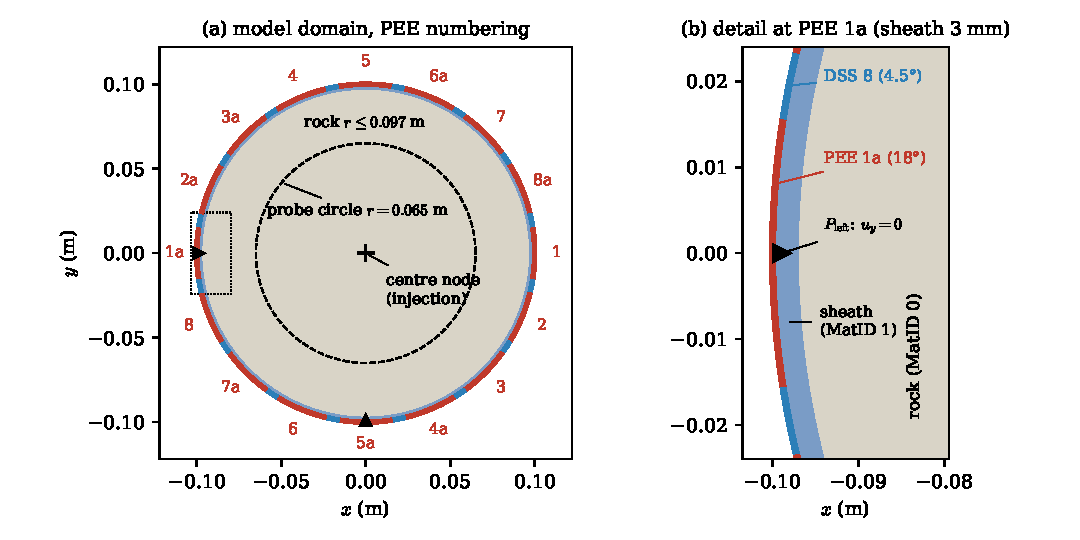
\includegraphics[width=\textwidth]{figures/fig_geometry.pdf}
\caption{Model geometry. (a) Rock disc, sheath, PEE arcs (red, numbered) and
DSS arcs (blue), probe circle (dashed), centre node and rigid-body points
(triangles). (b) Detail of the rock--sheath boundary at PEE~1a.}
\label{fig:geometry}
\end{figure}

\subsection{Mesh}
The mesh is generated with Gmsh (\texttt{make\_great\_cell\_mesh.py}) and has
11\,889 nodes and 5\,804 quadratic triangles (Fig.~\ref{fig:mesh}). Element size
is \SI{1.5}{mm} at the centre, \SI{6}{mm} at the probe circle and \SI{2}{mm} in
the sheath. Displacement uses quadratic, pressure and temperature linear shape
functions (Taylor--Hood).

\begin{figure}[htbp]
\centering
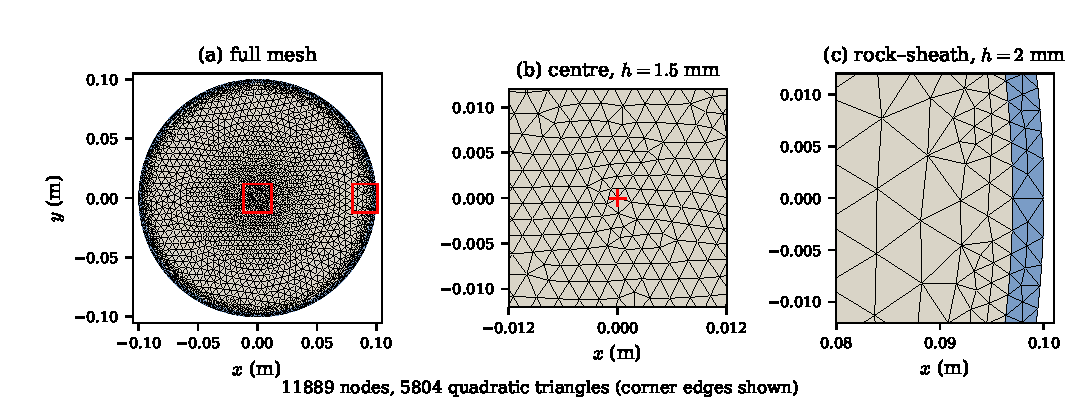
\includegraphics[width=\textwidth]{figures/fig_mesh.pdf}
\caption{Finite element mesh. (a) Full mesh with the two detail windows (red).
(b) Refinement around the injection node. (c) Rock--sheath transition.}
\label{fig:mesh}
\end{figure}

\subsection{Boundary and initial conditions}
Table~\ref{tab:bc} and Fig.~\ref{fig:bc} summarise the conditions. Load~A
(Table~4 of~\cite{Mollaali2026}) is applied as normal traction in the first
time step; each DSS carries the mean of its two neighbouring PEEs,
$\sigma_{\mathrm{DSS},i} = (\sigma_{\mathrm{PEE},i}+\sigma_{\mathrm{PEE},i+1})/2$.

\begin{table}[htbp]
\centering
\caption{Boundary and initial conditions of the THM model, Load A.}
\label{tab:bc}
\begin{tabularx}{\textwidth}{@{}lL@{}}
\toprule
Item & Setting \\
\midrule
PEE tractions (MPa)  & PEE 1--8 (and 1a--8a): 10.0, 6.64, 4.46, 1.17, 1.0, 3.82, 7.80, 9.95 \\
DSS tractions        & Mean of neighbouring PEEs \\
Rigid-body control   & $P_\mathrm{bottom}=(0,\,-0.09894)$: $u_x=u_y=0$; $P_\mathrm{left}=(-0.09894,\,0)$: $u_y=0$ \\
Out-of-plane         & Plane strain \\
Temperature          & Outer boundary: \SI{293}{K} $\rightarrow$ \SI{363}{K} linearly over \SIrange{0}{325}{s}, then held \\
Pressure             & Outer boundary drained, $p=p_0=\SI{1}{MPa}$ \\
Injection            & Centre node, \SIrange{4000}{4050}{s}: \SI{1}{l/min} $=\SI{1.667e-5}{m^3\,s^{-1}}$ per m (mass rate \SI{1.667e-2}{kg\,s^{-1}} per m), $T_\mathrm{inj}=\SI{293}{K}$ \\
Shut-in              & \SIrange{4050}{5000}{s} \\
Initial state        & $T_0=\SI{293}{K}$, $p_0=\SI{1}{MPa}$, $\mathbf{u}_0=\mathbf{0}$; initial effective stress $\alpha_B p_0$ so that total stress is zero \\
\bottomrule
\end{tabularx}
\end{table}

\begin{figure}[htbp]
\centering
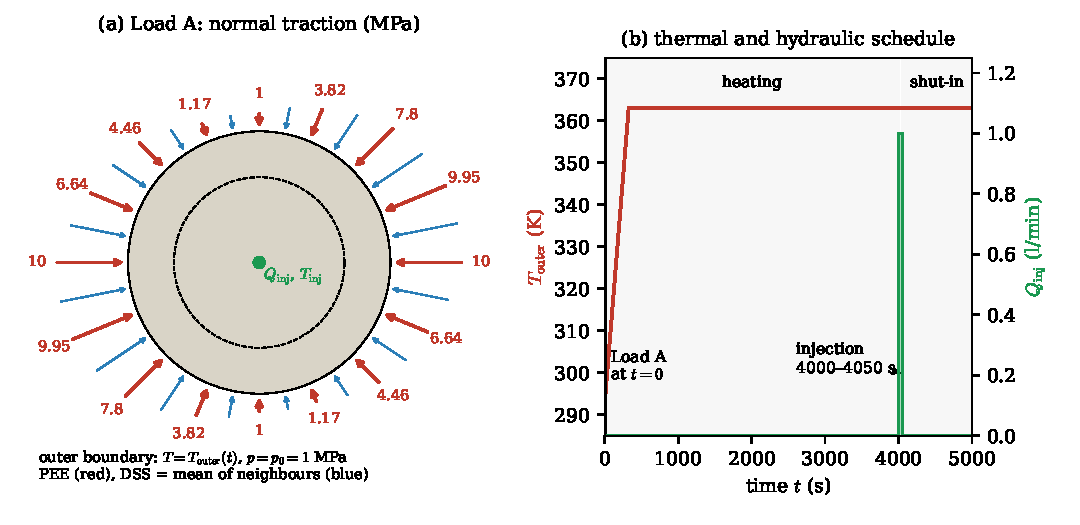
\includegraphics[width=\textwidth]{figures/fig_bc.pdf}
\caption{Boundary conditions. (a) Load A: normal traction on the PEEs (red,
values in MPa) and DSSs (blue); arrow length scales with traction. (b) Outer
boundary temperature and injection rate over time.}
\label{fig:bc}
\end{figure}

Time steps are \SI{5}{s} (\SIrange{0}{400}{s}), \SI{40}{s} (to \SI{4000}{s}),
\SI{1}{s} during injection, \SI{2}{s} (to \SI{4150}{s}) and \SI{10}{s} (to
\SI{5000}{s}).

% ---------------------------------------------------------------
\section{Numerical implementation in OpenGeoSys}
% ---------------------------------------------------------------
All stages run in OpenGeoSys~6 (OGS) with the finite element method, monolithic
Newton--Raphson coupling and implicit Euler time stepping
(Table~\ref{tab:ogs}).

\begin{table}[htbp]
\centering
\caption{OGS processes per stage type.}
\label{tab:ogs}
\begin{tabularx}{\textwidth}{@{}lLL@{}}
\toprule
Stage type & OGS process & Fracture treatment \\
\midrule
Mechanics only              & \texttt{SMALL\_DEFORMATION} & None or LIE \\
Hydro-mechanics, intact     & \texttt{HYDRO\_MECHANICS} & None \\
Hydro-mechanics, fractured  & \texttt{HYDRO\_MECHANICS} with LIE & Discrete lower-dimensional interface elements \\
Fracture propagation        & Phase-field (VPF) HM coupling & Smeared, AT1/AT2 \\
Thermo-hydro-mechanics      & \texttt{THERMO\_HYDRO\_MECHANICS} (or TH2M, saturated) & None or LIE \\
\bottomrule
\end{tabularx}
\end{table}

Displacements use quadratic elements and pressure and temperature linear ones
(Taylor--Hood) for stable pressure fields. Pre- and post-processing (load tables
per PEE, mesh generation, fibre-line extraction) run in Jupyter notebooks with
\texttt{ogstools}.

The reference THM runs use OGS~6.5.9 with \texttt{THERMO\_HYDRO\_MECHANICS}
(about 13~min per rock).

% ---------------------------------------------------------------
\section{The OGS project}
% ---------------------------------------------------------------
The THM model is defined by one OGS project file per rock,
\texttt{THM\_greywacke\_loadA.prj} and \texttt{THM\_gneiss\_loadA.prj}, in the
folder \texttt{THM\_model}. Both are written by \texttt{make\_THM\_prj.py}, so
loads and parameters are changed in the script, not in the XML. The two files
differ only in the rock parameters of medium~0.

\subsection{The OGS project file (PRJ)}
An OGS simulation is fully defined by one project file with the extension
\texttt{.prj}. It is a plain XML file with the root element
\texttt{<OpenGeoSysProject>} and is passed to the solver on the command line,
\texttt{ogs model.prj}. The file does not contain the mesh itself; it refers to
VTU meshes stored next to it. Its main blocks are:
\begin{itemize}[itemsep=0pt]
  \item \texttt{<meshes>} -- the bulk mesh and the boundary and point meshes on
        which conditions and outputs are defined;
  \item \texttt{<processes>} -- the physical process (here
        \texttt{THERMO\_HYDRO\_MECHANICS}), its process variables and the
        constitutive relations;
  \item \texttt{<media>} -- material properties per MaterialID and phase
        (liquid, solid, medium);
  \item \texttt{<time\_loop>} -- time stepping, coupling, convergence criteria and
        output;
  \item \texttt{<parameters>} and \texttt{<curves>} -- named constants, fields,
        functions and time curves used by the other blocks;
  \item \texttt{<process\_variables>} -- initial conditions, boundary conditions
        and source terms for each primary variable;
  \item \texttt{<nonlinear\_solvers>} and \texttt{<linear\_solvers>} -- the
        Newton and linear solver settings.
\end{itemize}
Blocks refer to each other by name; a boundary condition, for example, names a
mesh and a parameter. XML comments in the file document the model set-up.

\subsection{Files and workflow}
\begin{table}[htbp]
\centering
\caption{Files of the THM model (folder \texttt{THM\_model}).}
\label{tab:files}
\begin{tabularx}{\textwidth}{@{}lL@{}}
\toprule
File & Content \\
\midrule
\texttt{make\_great\_cell\_mesh.py} & Gmsh mesh and all OGS meshes (\texttt{domain.vtu}, subdomains with \texttt{bulk\_node\_ids}/\texttt{bulk\_element\_ids}); options \texttt{-{}-lc}, \texttt{-{}-lc\_sheath}, \texttt{-{}-lc\_center}, \texttt{-{}-order}, \texttt{-{}-w\_pee} \\
\texttt{make\_THM\_prj.py} & Writes the two project files; options \texttt{-{}-load} (A, B, C, E, F) and \texttt{-{}-alpha\_T} \\
\texttt{THM\_<rock>\_loadA.prj} & OGS project files \\
\texttt{plot\_THM\_overview.py} & Overview plot \texttt{THM\_loadA\_overview.png}: centre $T$ and $p$, radial profiles, $\varepsilon_\mathrm{vol}$ on the probe circle \\
\texttt{THM\_out\_loadA.zip} & Results and logs \\
\bottomrule
\end{tabularx}
\end{table}

The workflow is:
\begin{enumerate}
  \item \texttt{python make\_great\_cell\_mesh.py} -- mesh and subdomain meshes;
  \item \texttt{python make\_THM\_prj.py -{}-load A} -- project files;
  \item \texttt{ogs -o out THM\_greywacke\_loadA.prj} (and Gneiss) -- simulation,
        about 13~min per rock with OGS~6.5.9;
  \item \texttt{python plot\_THM\_overview.py} -- post-processing.
\end{enumerate}

\subsection{Structure of the project file}
Table~\ref{tab:prj} maps the XML sections of the project file to the model
components described above.

\begin{table}[htbp]
\centering
\caption{Sections of \texttt{THM\_greywacke\_loadA.prj}.}
\label{tab:prj}
\begin{tabularx}{\textwidth}{@{}lL@{}}
\toprule
XML section & Content \\
\midrule
\texttt{<meshes>} & 22 meshes: \texttt{domain}, \texttt{PEE\_1}--\texttt{PEE\_8}, \texttt{DSS\_1}--\texttt{DSS\_8} (each holds arcs $i$ and $i$a), \texttt{outer\_boundary}, \texttt{fix\_bottom}, \texttt{fix\_left}, \texttt{center}, \texttt{probe\_circle} \\
\texttt{<processes>} & \texttt{THERMO\_HYDRO\_MECHANICS}, integration order 4; constitutive relation \texttt{LinearElasticIsotropic} per MaterialID (0 rock, 1 sheath); \texttt{equation\_balance\_type = mass}; \texttt{initial\_stress = sigma0}; no gravity; secondary variables $\bm{\sigma}$, $\bm{\varepsilon}$, Darcy velocity \\
\texttt{<media>} & Medium 0 (rock) and 1 (sheath), each with an \texttt{AqueousLiquid} phase (density linear in pressure, slope $4.4\times10^{-10}$ Pa$^{-1}$ around 1~MPa; constant $\mu$, $c$, $\lambda$; no thermal expansion), a \texttt{Solid} phase ($\rho_s$, $\lambda_s$, $c_s$, $\alpha_T$) and medium properties ($k$, $\phi$, $\alpha_B$, \texttt{EffectiveThermalConductivityPorosityMixing}) \\
\texttt{<time\_loop>} & Newton with \texttt{PerComponentDeltaX} (NORM2; absolute tolerances $10^{-1}$~K, $10$~Pa, $10^{-7}$~m, $10^{-7}$~m); \texttt{BackwardEuler}; \texttt{FixedTimeStepping} \SIrange{0}{5000}{s} in five blocks (Table~\ref{tab:bc}); VTK output of \texttt{domain} at 14 fixed times, \texttt{center} and \texttt{probe\_circle} at every step \\
\texttt{<parameters>} & Material constants, \texttt{sigma0} per MaterialID ($\alpha_B p_0$ in the rock, 0 in the sheath), initial values \texttt{T0}, \texttt{p0}, \texttt{u0}, the 16 traction values \texttt{sigma\_PEE\_i}/\texttt{sigma\_DSS\_i}, \texttt{T\_outer} (\texttt{CurveScaled}), \texttt{T\_inj}, and \texttt{Q\_inj} (\texttt{Function}: \SI{16.67}{g\,s^{-1}} per m for $4000 < t \le 4050$~s) \\
\texttt{<curves>} & \texttt{T\_outer\_curve}: (0, 325, 5000)~s $\rightarrow$ (293, 363, 363)~K \\
\texttt{<process\_variables>} & \texttt{temperature} (order 1): Dirichlet \texttt{T\_outer} on \texttt{outer\_boundary}, \texttt{DirichletWithinTimeInterval} \texttt{T\_inj} on \texttt{center} (4000.5--4050~s); \texttt{pressure} (order 1): Dirichlet \texttt{p0} on \texttt{outer\_boundary}, nodal source \texttt{Q\_inj} on \texttt{center}; \texttt{displacement} (order 2): Dirichlet on \texttt{fix\_bottom} ($u_x$, $u_y$) and \texttt{fix\_left} ($u_y$), \texttt{NormalTraction} on the 16 PEE/DSS meshes \\
\texttt{<nonlinear\_solvers>} & Newton, at most 20 iterations \\
\texttt{<linear\_solvers>} & Eigen \texttt{SparseLU} with scaling \\
\bottomrule
\end{tabularx}
\end{table}

Two details are worth noting. First, the injection is a mass rate because the
process balances mass, which is needed for the pressure-dependent water
density. Second, the initial stress \texttt{sigma0} $=\alpha_B p_0$ makes the
initial state ($p=p_0$, no load) free of total stress, so the response is due
to Load~A, heating and injection only.


% ---------------------------------------------------------------
\section{Results}
% ---------------------------------------------------------------
The model was built in three steps of increasing coupling: a thermal (T)
model, a thermo-hydraulic (TH) model and the full THM model. Each step was
checked against an analytical solution or the previous step. All runs use
OGS~6.5.9. Table~\ref{tab:results} summarises the key numbers.

\begin{table}[htbp]
\centering
\caption{Key results of the T, TH and THM models.}
\label{tab:results}
\begin{tabularx}{\textwidth}{@{}llL@{}}
\toprule
Model & Quantity & Result \\
\midrule
T, step   & Max.\ error vs.\ Bessel series & \SI{0.47}{K} \\
T, ramp   & Max.\ error vs.\ Duhamel solution & \SI{0.15}{K} \\
TH        & $T$ at \SI{4000}{s} vs.\ T model & max.\ difference \SI{0.015}{K} \\
TH        & Pressure vs.\ Thiem solution & within 0.2\,\%; $\Delta p = \SI{1.09}{MPa}$ at the centre node, \SI{0.078}{MPa} at $r=\SI{0.066}{m}$ \\
TH        & Cooling front at \SI{4050}{s}; centre $T$ at \SI{5000}{s} & $\sim$\SI{2}{cm}; \SI{353.7}{K} \\
THM       & Centre $T$ at 4000 / 4050 / 4100 / 5000~s & 356.7 / 293.0 / 309.5 / 353.6~K (both rocks) \\
THM       & Max.\ $\Delta p$ at the centre node & \SI{1.12}{MPa} (both rocks); \SI{0.081}{MPa} at $r=\SI{0.065}{m}$ (Thiem: 0.0811) \\
THM       & Mean $\varepsilon_\mathrm{vol}$ on probe circle, Greywacke & $-2.46$ (5~s), 11.15 (4000~s), 10.73 (4460~s), 10.94 (5000~s) $\times10^{-2}$\,\% \\
THM       & Mean $\varepsilon_\mathrm{vol}$ on probe circle, Gneiss & $-0.95$ (5~s), 12.03 (4000~s), 11.62 (4450~s), 11.82 (5000~s) $\times10^{-2}$\,\% \\
\bottomrule
\end{tabularx}
\end{table}

\subsection{T model}
The T model (\texttt{HEAT\_CONDUCTION}) solves heat conduction in a granite
disc of radius \SI{0.1}{m} ($\rho=\SI{2700}{kg\,m^{-3}}$,
$\lambda=\SI{2.8}{W\,m^{-1}\,K^{-1}}$, $c_p=\SI{790}{J\,kg^{-1}\,K^{-1}}$) on a
mesh of 2\,991 nodes. Two cases were run from $T_0=\SI{293}{K}$: a step to
\SI{323}{K} at the outer boundary, and the linear ramp to \SI{363}{K} over
\SI{325}{s} used later in the THM model. OGS agrees with the analytical
solutions to within \SI{0.47}{K} (step) and \SI{0.15}{K} (ramp), and the time
discretisation converges with order $\sim$1, as expected for backward Euler
(Fig.~\ref{fig:T}). The centre reaches the boundary temperature after about
2~h for the step case.

\begin{figure}[htbp]
\centering
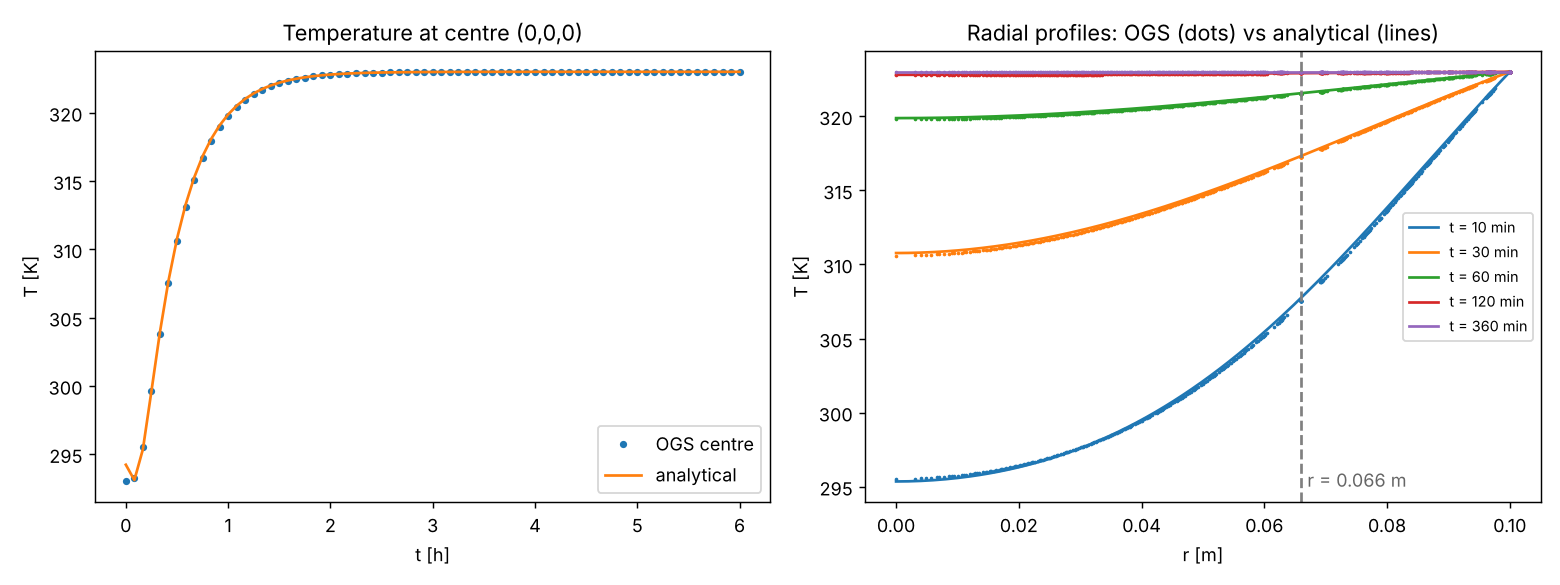
\includegraphics[width=\textwidth]{figures/fig_T_verification.png}
\caption{T model, step case: centre temperature over time (left) and radial
profiles (right); OGS (dots) vs.\ analytical solution (lines).}
\label{fig:T}
\end{figure}

\subsection{TH model}
The TH model (\texttt{HT}) adds Darcy flow and heat advection to the ramp case
($k=1.409\times10^{-14}$~m$^2$, $S=1.419\times10^{-11}$~Pa$^{-1}$, $\phi=0.01$).
Cold water (\SI{293}{K}) is injected at the centre at \SI{1}{l/min} per metre
from 4000 to \SI{4050}{s}, followed by shut-in (Fig.~\ref{fig:TH}).

\begin{itemize}
  \item \textbf{Heating phase.} Before injection the TH model reproduces the T
        model within \SI{0.015}{K}; the centre reaches \SI{356.7}{K} at
        \SI{4000}{s}.
  \item \textbf{Pressure.} The pressure diffusivity $k/(\mu S)\approx\SI{1}{m^2/s}$
        makes the pressure response quasi-instantaneous: the profile becomes the
        steady Thiem solution within \SI{0.1}{s} and drops back to $p_0$ at
        shut-in. The centre node reaches $\Delta p=\SI{1.09}{MPa}$.
  \item \textbf{Cooling.} Injection cools the centre to \SI{293}{K} and pushes a
        cooling front about \SI{2}{cm} into the disc by \SI{4050}{s}. After
        shut-in, conduction from the hot boundary reheats the centre to
        \SI{353.7}{K} at \SI{5000}{s}.
\end{itemize}

\begin{figure}[htbp]
\centering
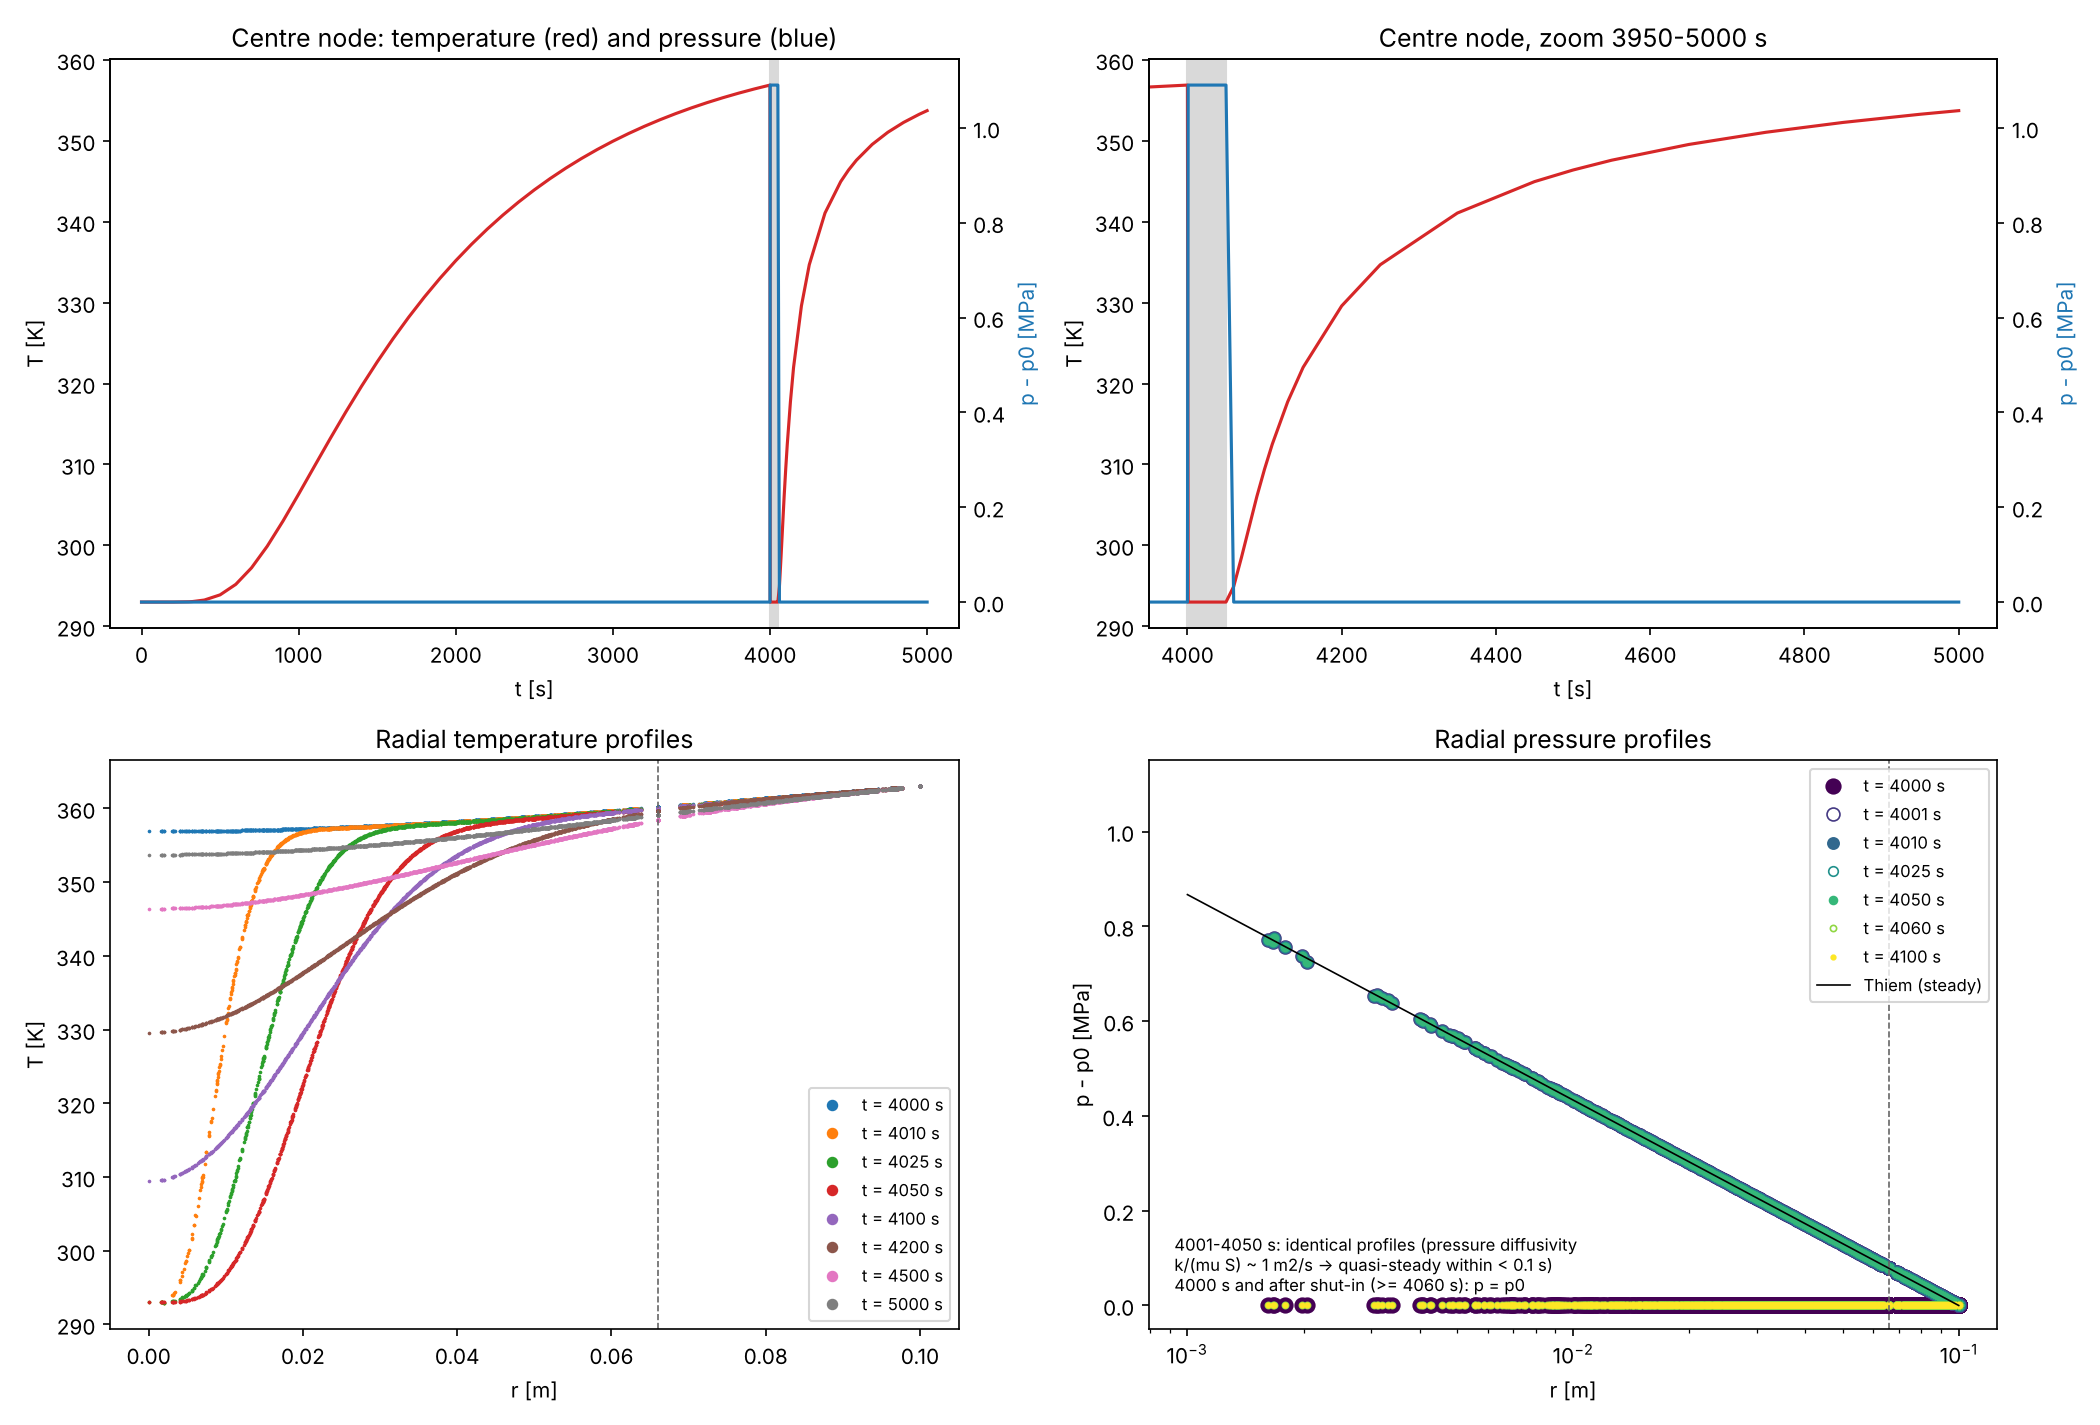
\includegraphics[width=\textwidth]{figures/fig_TH_overview.png}
\caption{TH model: centre temperature and pressure (top), radial temperature
profiles (bottom left) and radial pressure profiles with the Thiem solution
(bottom right).}
\label{fig:TH}
\end{figure}

\subsection{THM model}
The THM model combines the TH set-up with Load~A on the GREAT cell geometry for
Greywacke and Gneiss (Fig.~\ref{fig:THM}).

\begin{itemize}
  \item \textbf{Temperature and pressure.} Both rocks give the same centre
        temperature (356.7~K at \SI{4000}{s}, 353.6~K at \SI{5000}{s}) and the
        same injection pressure (\SI{1.12}{MPa} at the centre node), because
        permeability and bulk thermal properties are equal. The centre
        temperature differs from the TH model by at most \SI{0.42}{K}, caused
        by the larger time steps during heating. The pressure at
        $r=\SI{0.065}{m}$ matches the Thiem solution (0.0812 vs.\
        \SI{0.0811}{MPa}).
  \item \textbf{Mechanical loading.} Load~A compresses the sample:
        mean $\varepsilon_\mathrm{vol}$ on the probe circle at \SI{5}{s} is
        $-2.46\times10^{-2}$\,\% (Greywacke) and $-0.95\times10^{-2}$\,\%
        (Gneiss). The strain varies with angle with two maxima near \ang{100} and
        \ang{280}, and matches the M1 model to within $0.01\times10^{-2}$\,\%.
  \item \textbf{Heating.} Thermal expansion dominates after a few hundred
        seconds. At \SI{4000}{s} ($\Delta T\approx\SI{67}{K}$ on the probe
        circle) mean $\varepsilon_\mathrm{vol}$ is $11.15\times10^{-2}$\,\%
        (Greywacke) and $12.03\times10^{-2}$\,\% (Gneiss), equal to the
        analytical estimate $2(1+\nu)\alpha_T\Delta T+\varepsilon_\mathrm{mech}$.
        The thermal part is larger for Greywacke (13.6 vs.\ $13.0\times10^{-2}$\,\%,
        higher $\nu$), but the stiffer Gneiss carries a smaller mechanical
        contraction, so its net strain is higher.
  \item \textbf{Injection.} Cold-water injection causes a small contraction of
        about $0.4\times10^{-2}$\,\% in both rocks, with a minimum at about
        \SI{4450}{s}, before the strain recovers with reheating. The angular
        pattern of the load is preserved throughout.
\end{itemize}

\begin{figure}[htbp]
\centering
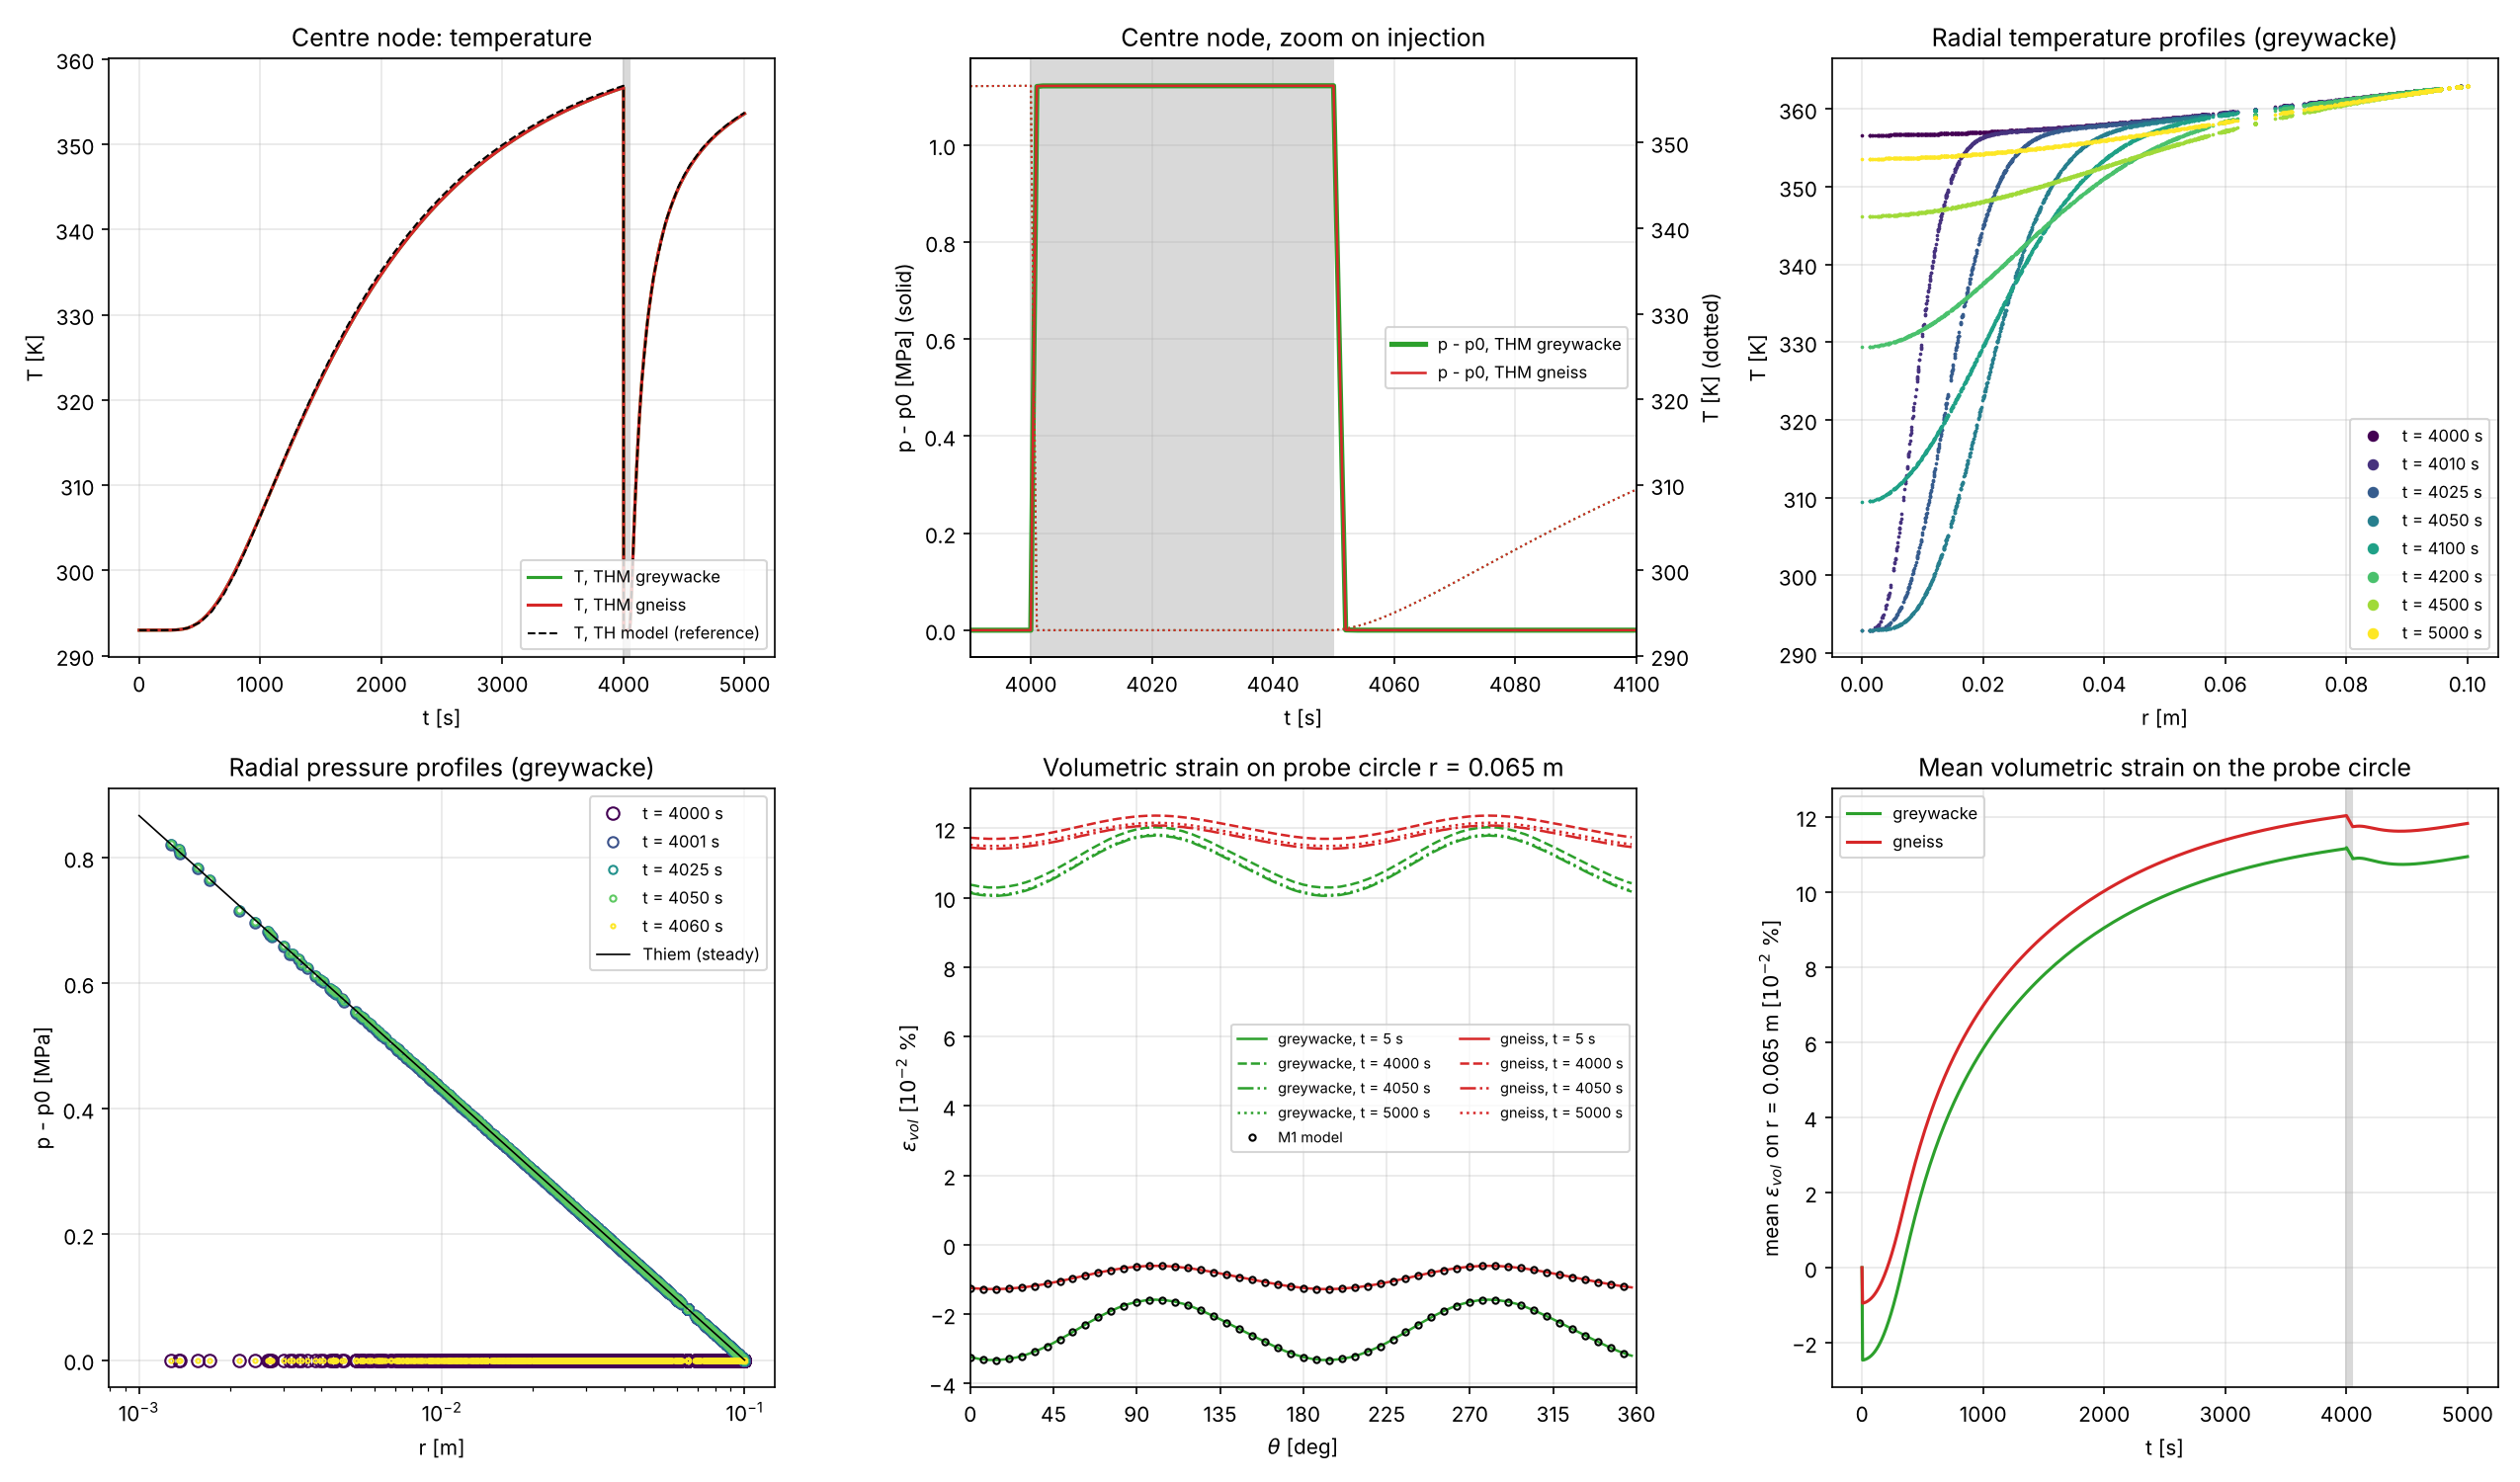
\includegraphics[width=\textwidth]{figures/fig_THM_overview.png}
\caption{THM model, Load~A: centre temperature compared with the TH model,
centre pressure during injection, radial temperature and pressure profiles
(Greywacke), volumetric strain on the probe circle vs.\ angle (with the M1
model at \SI{5}{s}), and mean volumetric strain over time.}
\label{fig:THM}
\end{figure}


% ---------------------------------------------------------------
\section{Benchmark stages and validation}
% ---------------------------------------------------------------
The stages add one coupling at a time, so each code's error can be traced to a
single process.
\begin{enumerate}
  \item \textbf{Intact, mechanical:} Greywacke and Gneiss under Loads A--C,
        rotated \ang{0}--\ang{90} in \ang{22.5} steps. Output: circumferential
        strain along the fibre and volumetric strain inside $r=\SI{0.065}{m}$.
  \item \textbf{Intact, hydro-mechanical:} \SI{3000}{s} mechanical
        equilibration, then \SI{500}{s} borehole injection (end at \SI{3500}{s}).
        Output: pressure and strain fields.
  \item \textbf{Static fracture, M and HM:} full and half fractures, with and
        without inflow--outflow. Output: aperture, fracture permeability versus
        normal stress as the load rotates.
  \item \textbf{Fracture propagation:} injection into a pre-existing fracture,
        and nucleation from the borehole. Output: path, breakdown pressure,
        opening.
  \item \textbf{Thermal stages (THM):} heating of the sample by the cell bands,
        then cooling, under constant polyaxial load. Output: thermal strain and
        change of fracture permeability.
\end{enumerate}

Results so far: discrete (LIE) and smeared (VPF) methods give similar volumetric
strain for intact samples, and fracture permeabilities within one order of
magnitude~\cite{Mollaali2026}. Gneiss deforms less than Greywacke; injection into
Greywacke spreads strain widely, while Gneiss shows local pressure build-up. The
first experiments showed that \SIrange{20}{30}{\celsius} heating closed the
fracture plastically and lowered its permeability~\cite{McDermott2018}.

Validation compares simulated surface strain with the fibre-optic profiles at
the mid-height of the sample, and simulated injection pressures with the pump
records.

% ---------------------------------------------------------------
\section{Assumptions, limitations and open points}
% ---------------------------------------------------------------
\begin{itemize}
  \item \textbf{2D plane strain} ignores axial load variation, platen friction
        and end effects; the fibre sits at mid-height, where this is most valid.
  \item \textbf{Linear elasticity} cannot capture the plastic fracture closure
        seen on heating, or micro-cracking near the borehole.
  \item \textbf{Sheath stiffness} controls how PEE pressures reach the rock; its
        value strongly affects simulated strain.
  \item \textbf{Full saturation and single-phase flow} are assumed; air in the
        pore space during early injection is ignored.
  \item \textbf{Thermal stages} are the least constrained: heat losses through
        platens and the frame are not yet measured.
  \item \textbf{Open:} the fracture-outlet back pressure is reported as
        \SI{3.45}{MPa} in the methods and $\sim$\SI{3.2}{MPa} in the results
        of~\cite{McDermott2018}; the benchmark uses \SI{3.45}{MPa}.
\end{itemize}

% ---------------------------------------------------------------
\bibliographystyle{unsrtnat}
\bibliography{references}

\end{document}
